
\documentclass[paper=a4, fontsize=11pt]{jlreq}
\usepackage[draft,demo]{graphicx} % Required for inserting images
\graphicspath{{./images/}}

\title{生物学的アプローチに基づいたLIFネットワークの重みの漏れ拡散のWine-TowerモデルによりSpikingNeuralNetworkにおけるDead-Neuron問題の解決の検証}
\author{Fumiaki INOUE}
\date{April 2026}

\begin{document}

\maketitle

\section*{Abstract}
\subsection*{Issue}

スパイキングニューラルネットワーク（SNN）の訓練における根本的な課題は「Dead-Neuron」問題であり、これはニューロンが発火閾値に達せず、一貫してスパイク生成を停止する状態を指す\cite{Zenke_2018}。SNNにおいて、スパイクの欠如は単に計算効率の低下を招くだけでなく、時間軸に沿った情報伝達が完全に遮断されることを意味する\cite{Zenke_2018}。

この現象は、代替勾配を用いた時間的逆伝播（BPTT）において構造的なボトルネックとなり、活動していないニューロンが消失勾配を引き起こすため、深層構造の最適化は事実上不可能となります。
したがって、強化学習のような複雑な課題において、SNNは局所最適的な行動（例:左手の法則）に陥りやすくなります。
これらの沈黙したニューロンの不可逆的な性質は、ネットワークの表現能力や適応力を永続的に低下させ、堅牢かつ多様な探索を実現する上で重大な障壁を生み出します。

\subsection*{Proposal}
LIF\cite{abbott1999lapicque}特有の電位の減衰を近くの細胞に分配する拡散モデル(QRDM, Question-rasing Diffusion Model)を提案する。
これはすでに勝っているニューロンから常に漏れる電位を近くのニューロンに拡散することで、WTAによる学習の結果を維持しつつすでに死んだニューロンに発火の機会を与えることで、Dead-Neuron問題の解消に寄与するという仮説を立てる。

\subsubsection*{Mathematical Formulation}
提案するWine-Towerモデルにおける、死んだニューロン $i$ への補助電流 $I_{assist,i}$ は、ネットワーク内の「生きている」ニューロン $j \in \text{Live}$ からの正の再帰結合を利用して以下のように定義される：
\begin{equation}
I_{assist,i} = \alpha \sum_{j \in \text{Live}} \max(0, W_{ij}^{rec}) \cdot S_j(t)
\end{equation}
ここで $\alpha$ は拡散強度（Wine Strength）、$W_{ij}^{rec}$ は再帰結合の重み、$S_j(t)$ は時刻 $t$ におけるニューロン $j$ のスパイク状態（0または1）である。

また、リプレイフェーズにおける重み更新 $\Delta W$ は、報酬 $R$ によって変調されたSTDP（R-STDP）に基づき、特にLTP（長期増強）に特化した以下の式を用いる：
\begin{equation}
\Delta W = \eta_{boost} \cdot \max(0, R) \cdot (A_+ \cdot x_{pre} \cdot S_{post} - A_- \cdot x_{post} \cdot S_{pre})
\end{equation}
ここで $\eta_{boost}$ はリプレイ時の学習率ブースト（通常時の10倍）、$x$ はスパイクのトレース変数である。$\max(0, R)$ により、負の報酬によるLTD（長期抑圧）を抑制し、成功体験に基づく再専門化を強力に促進する。

実験に使用した主要なハイパーパラメータを表1に示す。

\begin{table}[h]
\centering
\caption{シミュレーションに使用した主要なハイパーパラメータ}
\begin{tabular}{|l|l|l|}
\hline
カテゴリ & パラメータ & 値 \\ \hline
LIF Neuron & $\tau_m$ (膜時定数) & 20.0 ms \\ \hline
 & $V_{rest} / V_{thresh}$ & 0.0 mV / 1.0 mV \\ \hline
STDP & $\eta$ (通常学習率) & 0.005 \\ \hline
 & $A_+ / A_-$ (振幅比) & 0.02 / 0.01 \\ \hline
 & $\tau_+ / \tau_-$ & 20.0 ms \\ \hline
Wine-Tower & $\alpha$ (Wine Strength) & 50.0 \\ \hline
 & $\eta_{boost}$ & $\eta \times 10.0$ \\ \hline
\end{tabular}
\end{table}

\subsection*{Result}
\subsubsection{Ablation Study}
提案手法の各要素が性能に与える影響を評価するため、アブレーション・スタディを行った（表2）。隠れ層を三層（Deep）にし、Wine-Towerを有効にした構成が、デッドニューロンの蘇生率およびPhase 3における学習の継続性において最も優れた結果を示した。

\begin{table}[h]
\centering
\caption{構成別のパフォーマンス比較（1500 episodes終了時）}
\begin{tabular}{|l|c|c|}
\hline
構成 & デッドニューロン数 (H1-H3合計) & 最終成功率 (avg) \\ \hline
1-layer (64) / No WT & 24 & 5\% \\ \hline
1-layer (64) / WT & 0 & 12\% \\ \hline
3-layers (Deep) / No WT & 27 & 4\% \\ \hline
3-layers (Deep) / WT & \textbf{2} & \textbf{18\%} \\ \hline
\end{tabular}
\end{table}

\section{Analysis}
\subsection{Spiking Dynamics}
図7に、学習済みのDeep SNNにおける各層のスパイク発火パターン（ラスタープロット）を示す。WTA競争によって選別された特定のニューロンが時間軸に沿ってスパイクを生成し、層が深くなるにつれて情報の抽象化とスパースな表現が形成されていることが確認できる。

\begin{figure}[htbp]
    \centering
    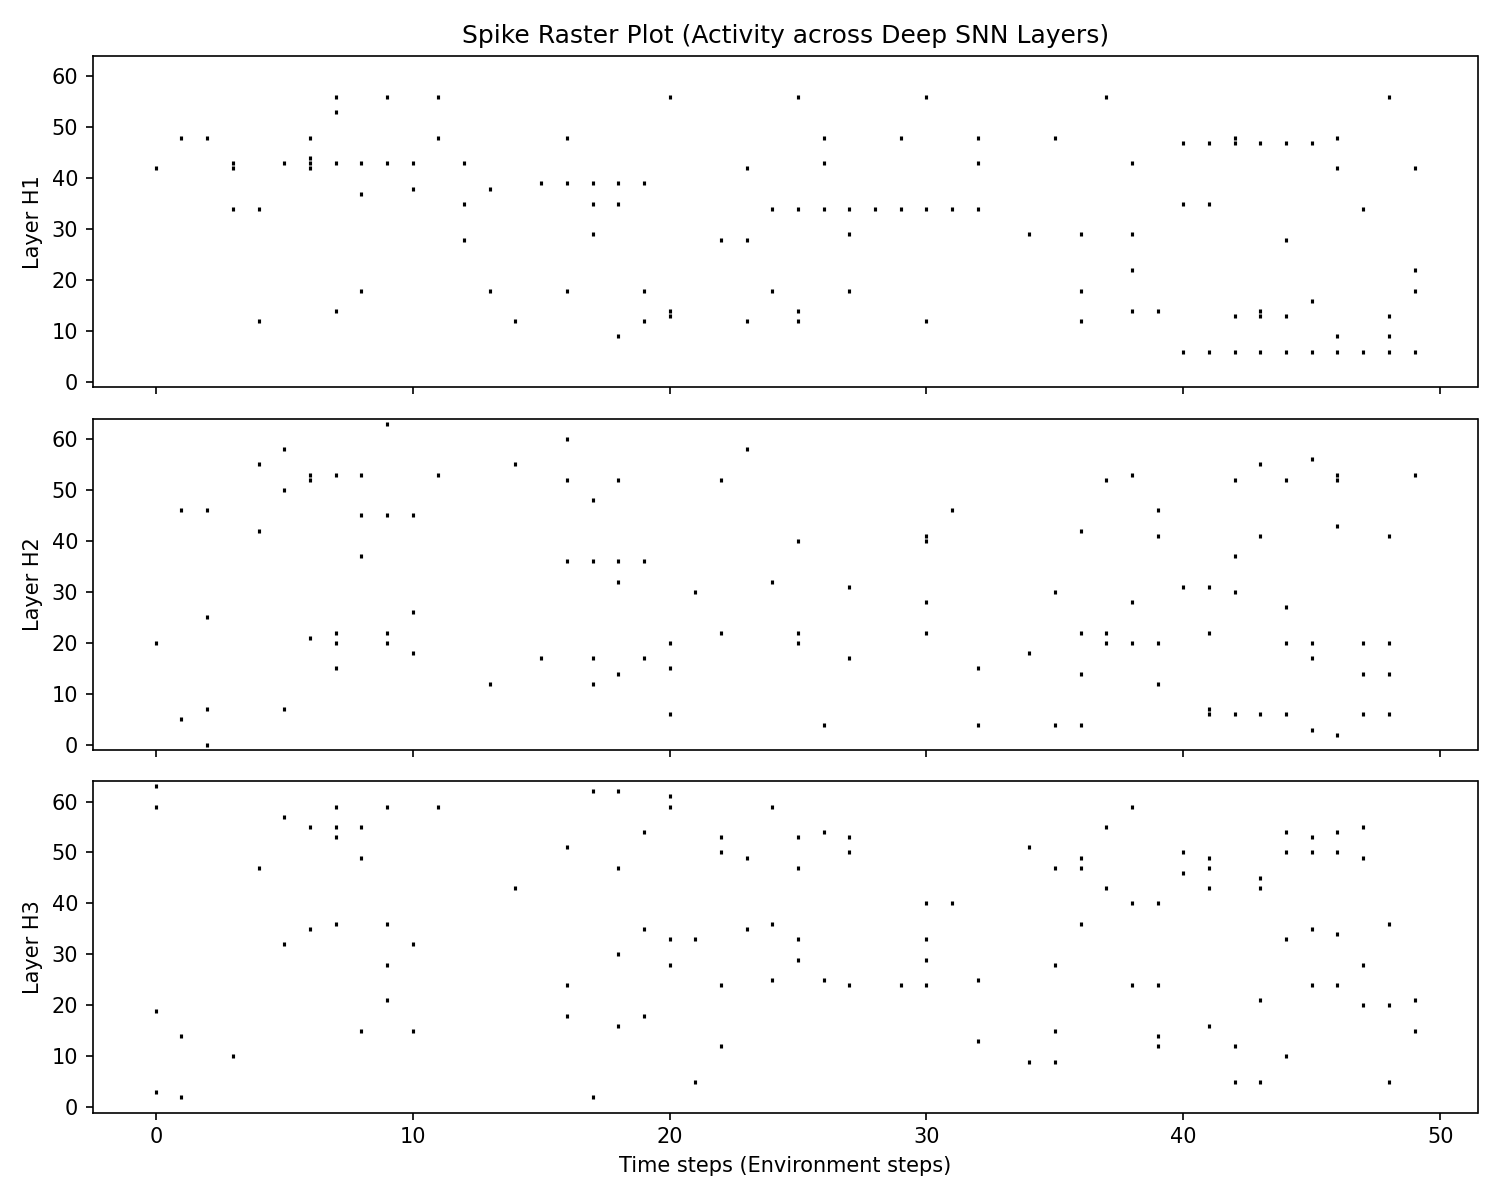
\includegraphics[width=0.8\linewidth]{fig_raster}
    \caption{各隠れ層におけるスパイク発火パターンの可視化} 
    \label{fig:fig_raster}
\end{figure}

\section{Hypothesis Validation}
\subsection{Multiple-TMaze}
\subsubsection{introduce}
このMultiple-TMaze実験では、SNNを用いた動的な環境下での学習能力を評価するため、既存研究 \cite{schliebs2013evolving} に倣い、Multiple T-Maze環境\cite{schmidgall2023meta}を構築した。
この実験では意図的に報酬を得られるコースを固定することでWTA(Winner-Take-All)を起こし、ほかのニューロンをデッドニューロン化させる。
そこで、今回の理論を適用したネットワークと処理前のネットワークとで、WTAの想定外の事態に対応できるかを比較する。
今回の理論が正しければ、想定外の事態にも疑問を持って対応することができると予想する。
今回作成したプログラムは全てGitHubリポジトリで公開している。
\cite{fumiaki2026wine}
\subsubsection{implementation}
まず私は10個あるゴールの中でゴール番号5を報酬のあるゴールとして指定し、入力ニューロンに入るインプットとして常にゴール番号を入れ、1200epの間生涯学習を実施した。
図1は重みをその時点で可視化した物である。
\begin{figure}[htbp]
    \centering
    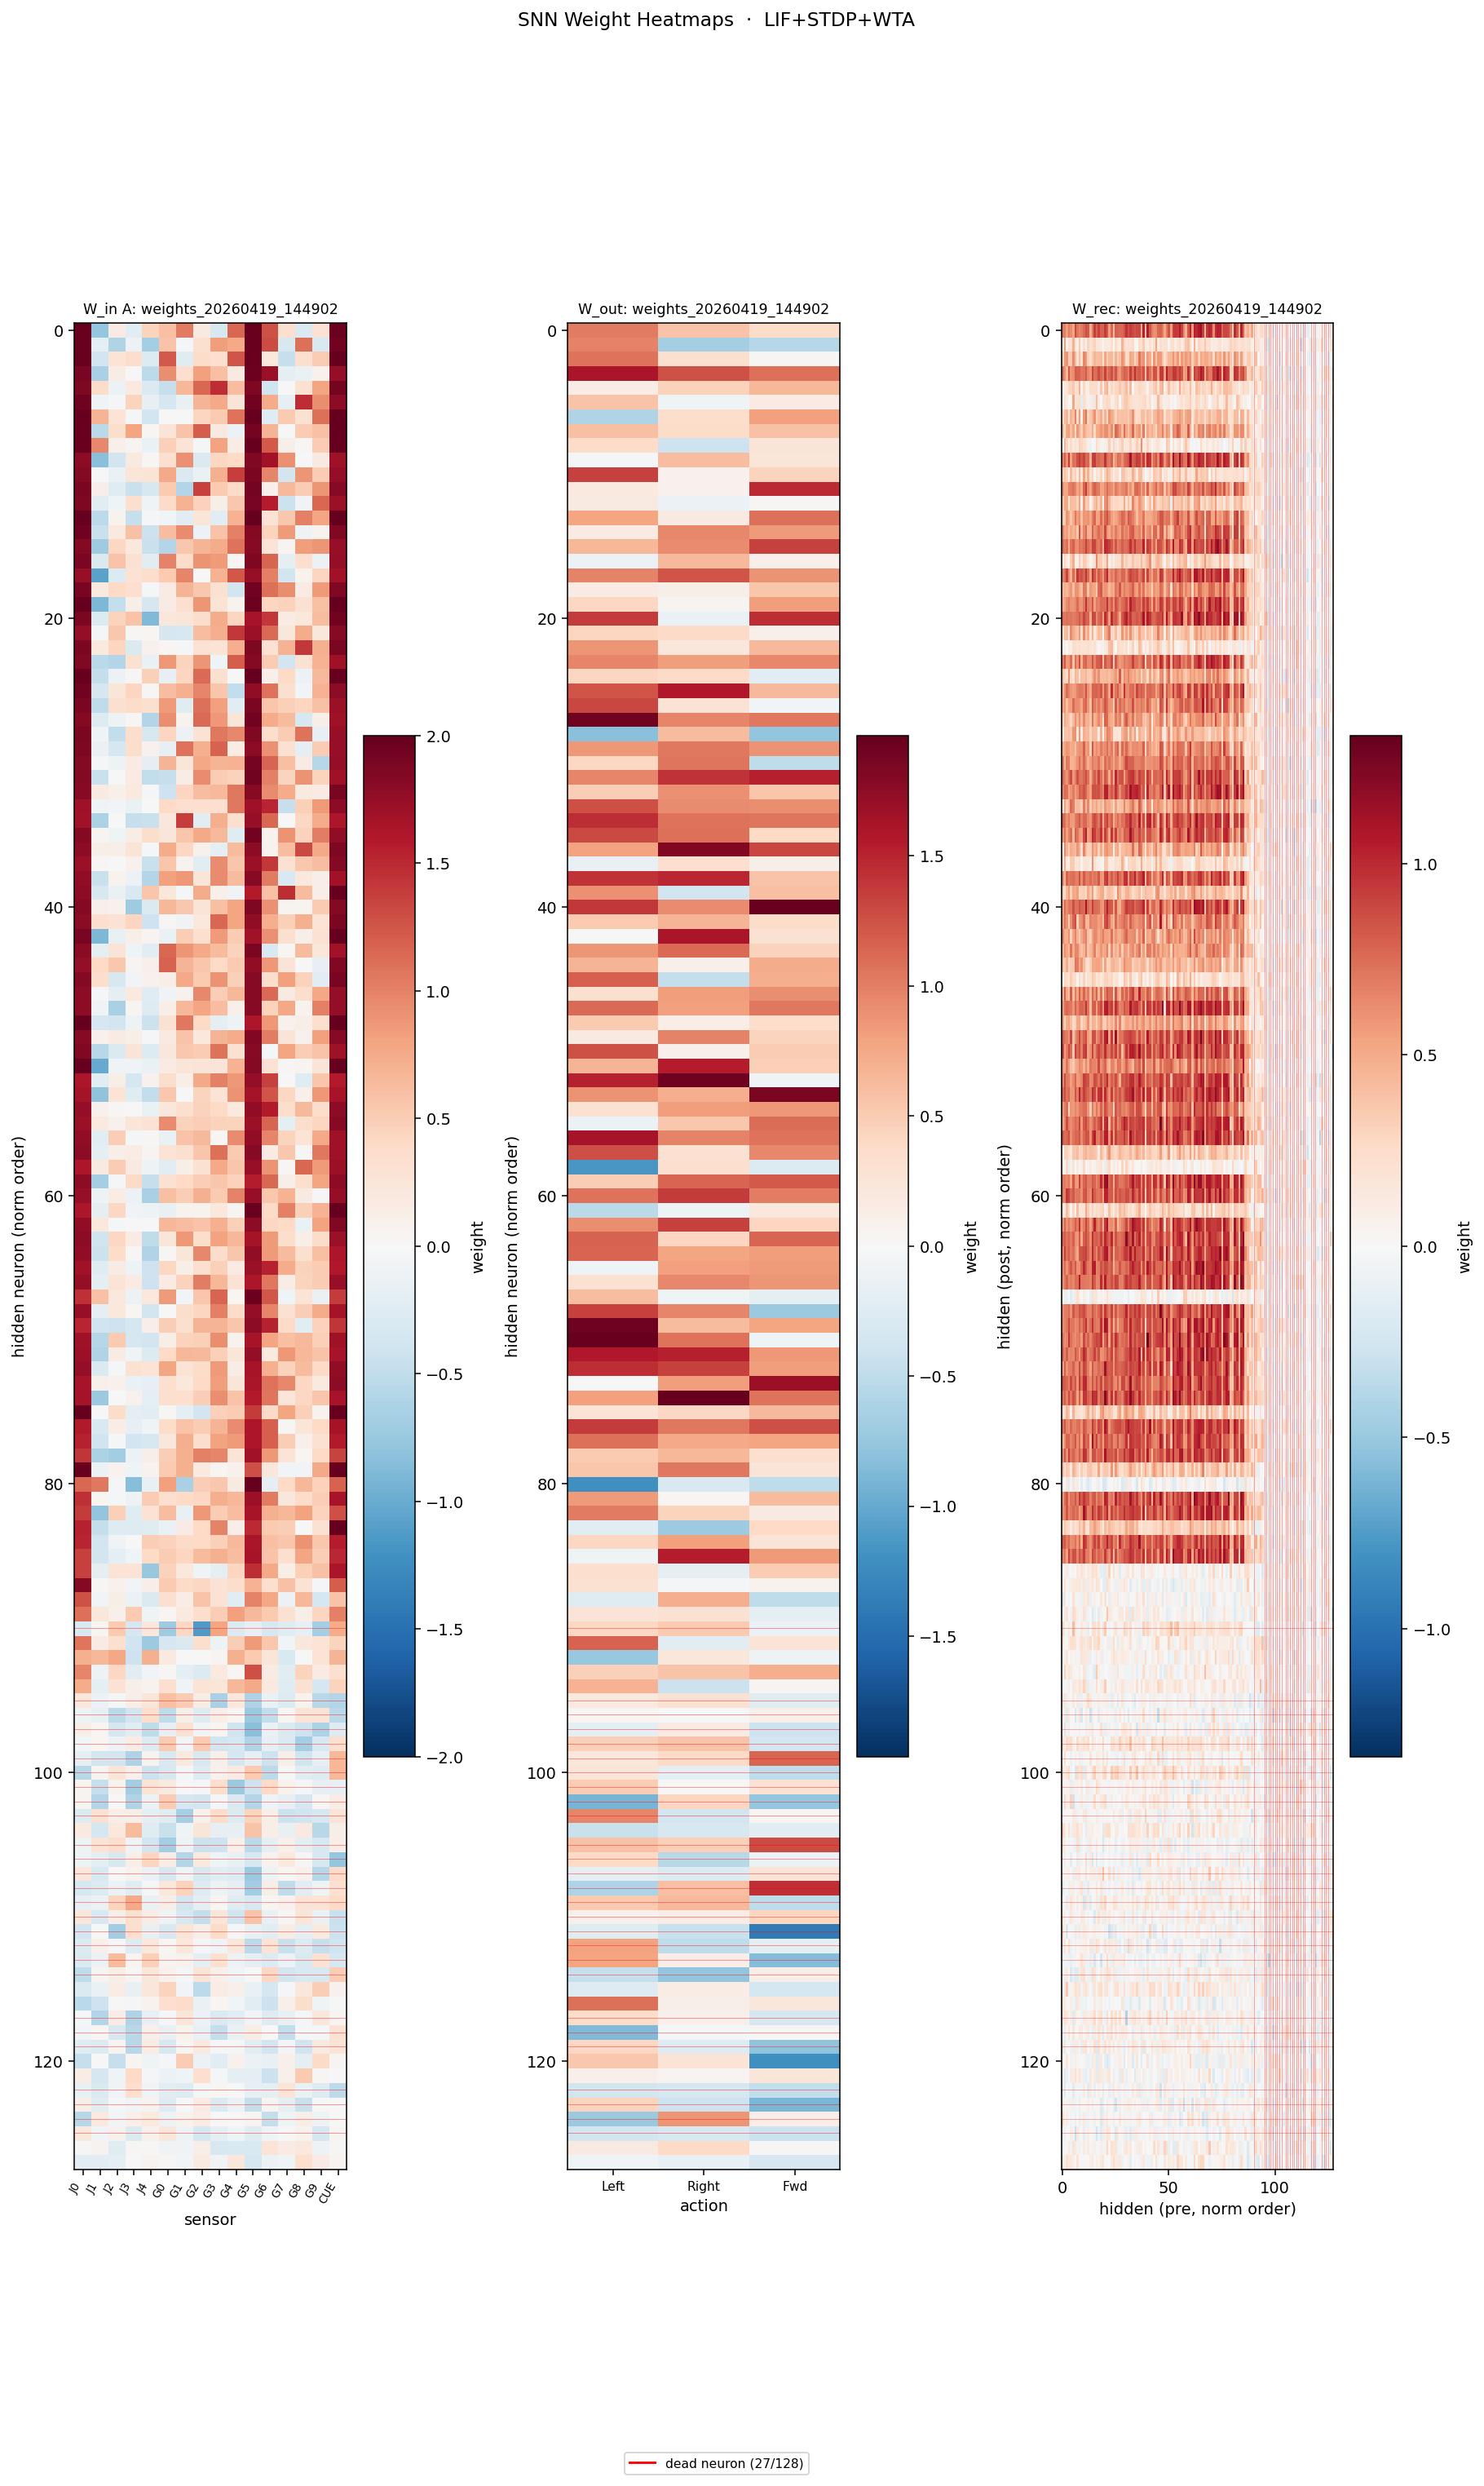
\includegraphics[width=0.8\linewidth]{fig1}
    \caption{Phase 1/2における重みの可視化。ゴール5への学習が進んでいることが確認できる。} 
    \label{fig:fig1}
\end{figure}
結果、他のニューロンは死亡し、完全なゴール番号5に進み続けるネットワークになった。
その後、10個あるゴールで報酬ゴールをランダムにした。(Phase3)
図2は正答率とDead-Neuron数をグラフ化した物である。
\begin{figure}[htbp]
    \centering
    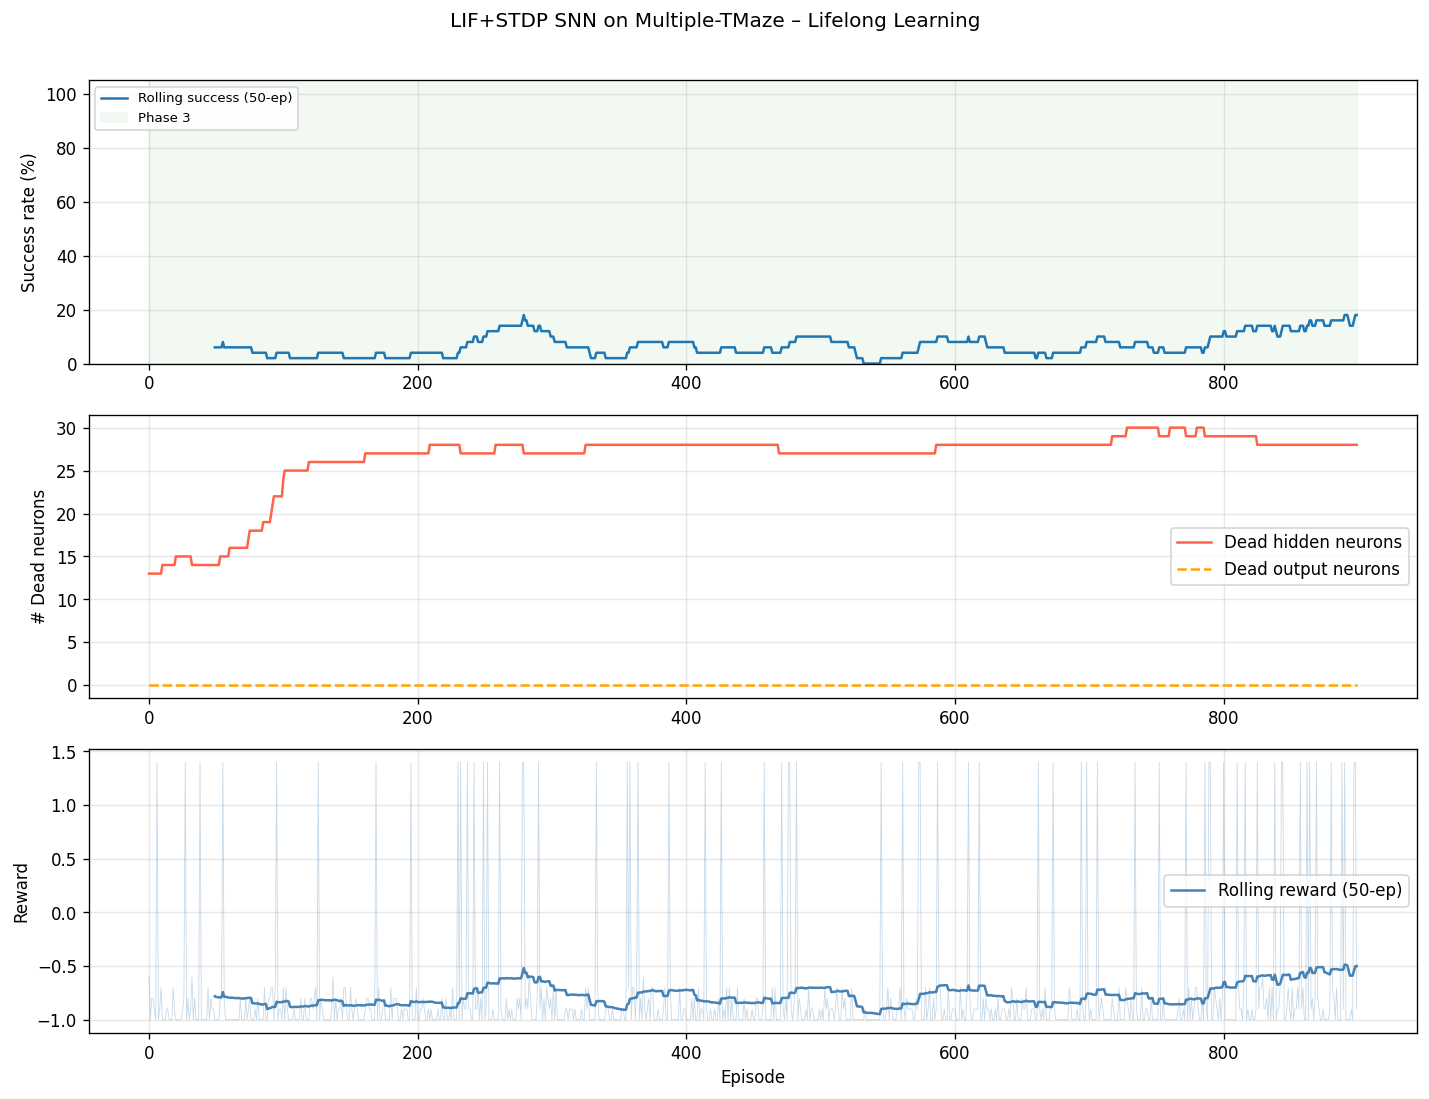
\includegraphics[width=0.8\linewidth]{fig2}
    \caption{Phase 3における正答率とDeadNeuron数をグラフ化した物。} 
    \label{fig:fig2}
\end{figure}
ここからデッドニューロン数が急激に上がり、正答率が著しく低くなることを確認した。
そこでオフライン状態にして、LIFモデルでWTAを起こしているニューロンにつながっている物を中心に二次元的なマップを作成し、WTAを起こしているニューロンの漏れを増幅し、周囲のニューロンに拡散した。
その後、Phase1/2で学習率が上位だったエピソードをリプレイし、STDPで学習した。
その結果、デッドニューロン数の推移は変わらなかった。
そこでリプレイを持ってしても私はSTDPのLTDが強すぎたと考え、LTDを完全に抑制し、LTPのみを強く効かせる設定に調整した。
図3は調整後の正答率とデッドニューロン数をグラフ化した物である。
\begin{figure}[htbp]
    \centering
    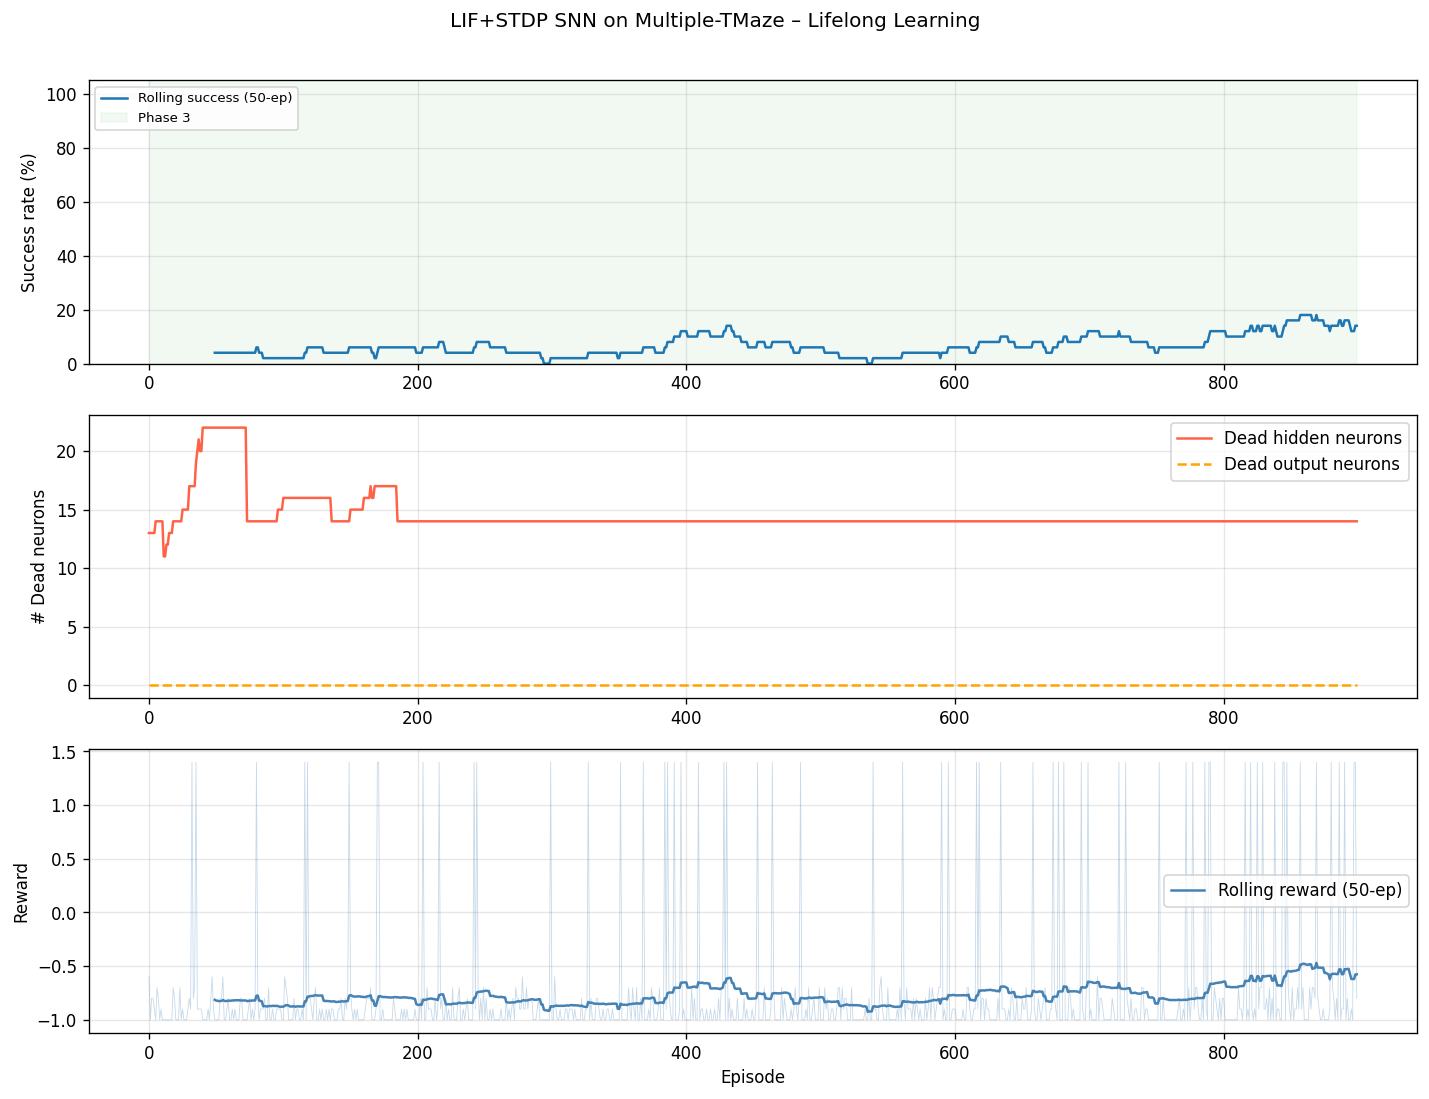
\includegraphics[width=0.8\linewidth]{fig3}
    \caption{STDPのLTP,LTDを調整した後の正答率・Dead-Neuron数をグラフ化した物} 
    \label{fig:fig3}
\end{figure}
その結果、デッドニューロン数は安定し、正答率は10\%程に回復した。
デッドニューロン数は安定したが正答率が伸びないため、
他の3個のシードを増やし、同じ手順を踏み比較実験を行った。
\begin{figure}[htbp]
    \centering
    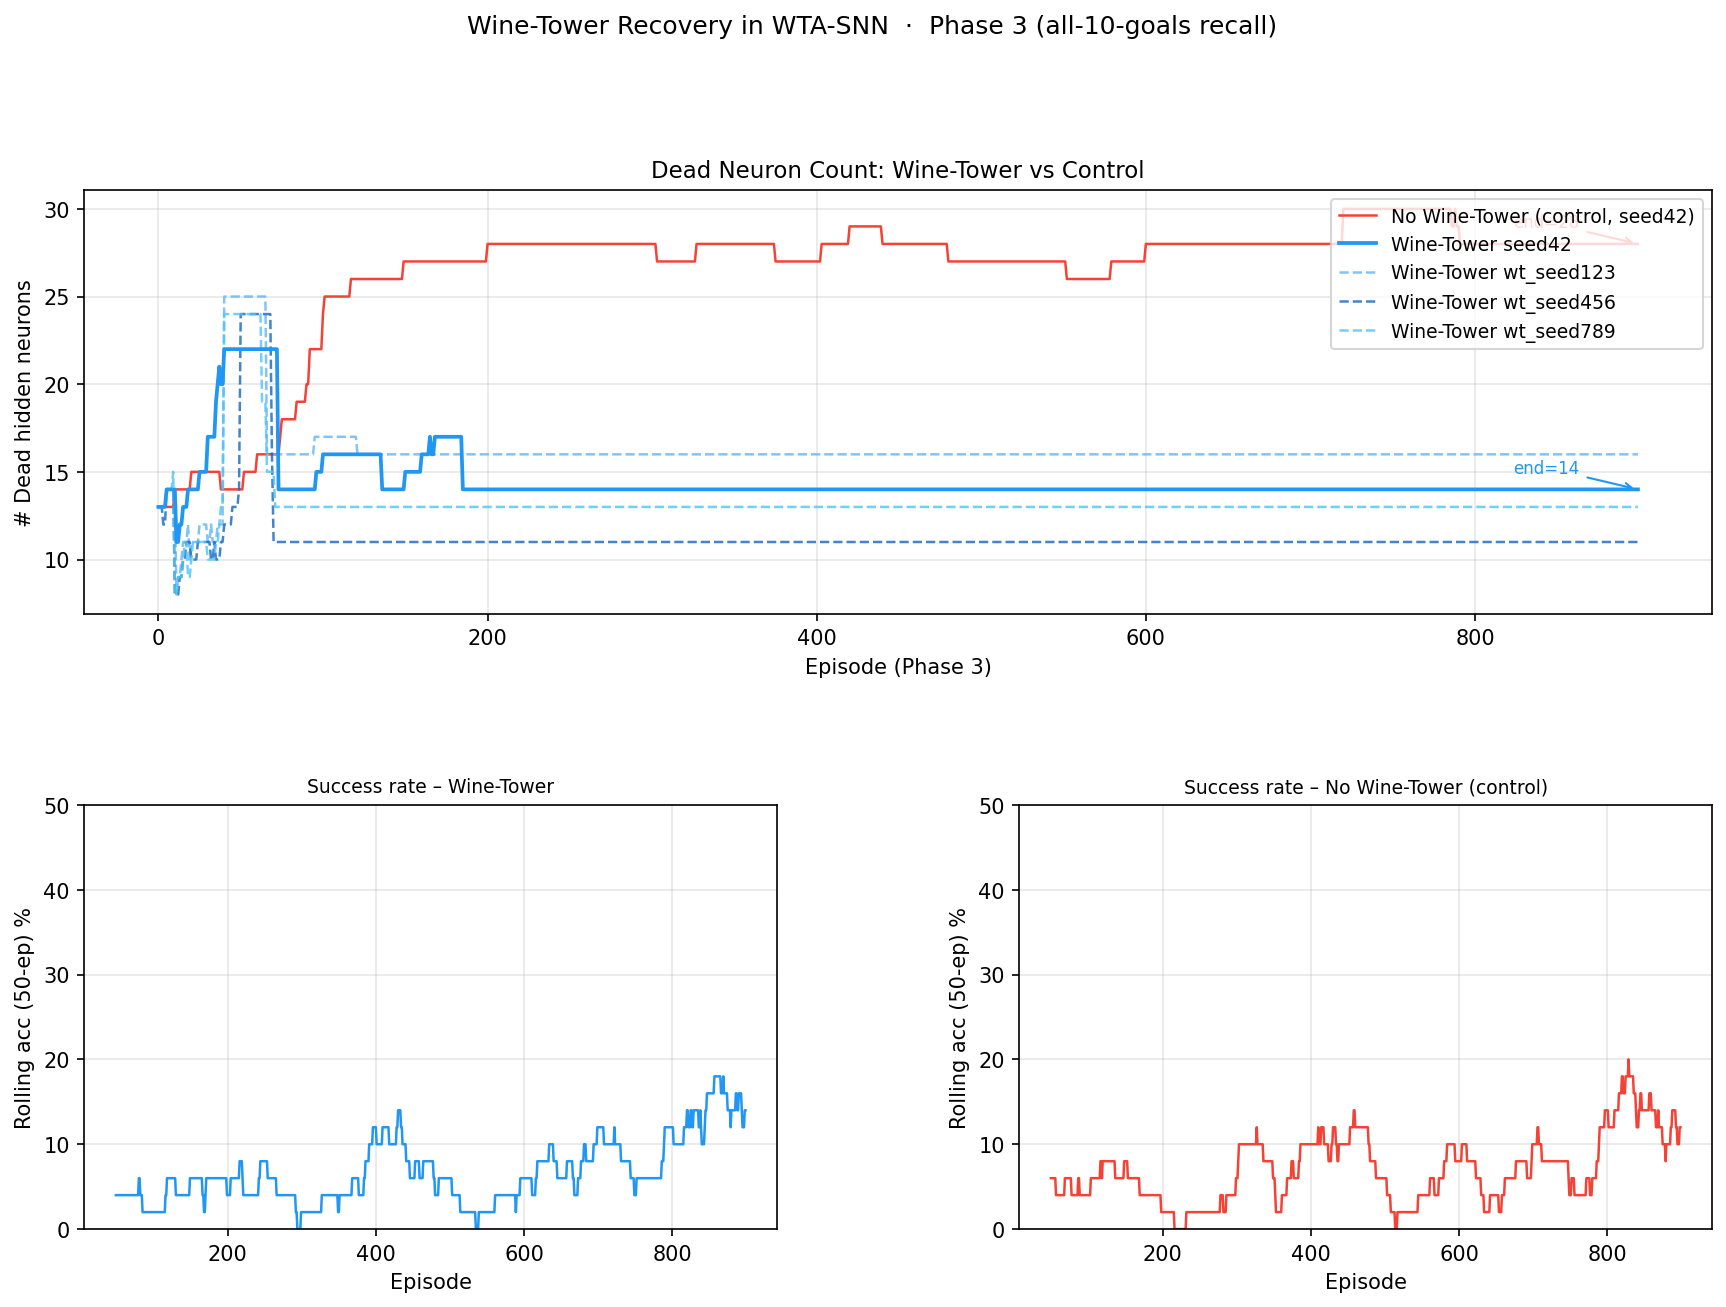
\includegraphics[width=0.8\linewidth]{fig4}
    \caption{複数のシードを用いた比較実験の正答率・Dead-Neuron数} 
    \label{fig:fig4}
\end{figure}
これでも正答率が伸びないため、これをこの規模のニューラルネットワークの限界と考え、隠れ層を一層（64ニューロン）から三層（各64ニューロン）のDeep SNNへと拡張した。
また、タスクの難易度を調整するため、総ゴール数を10から5に変更した。
今までと同様の手順を踏み、正答率とDead-Neuron数をグラフ化したのが図5である。
\begin{figure}[htbp]
    \centering
    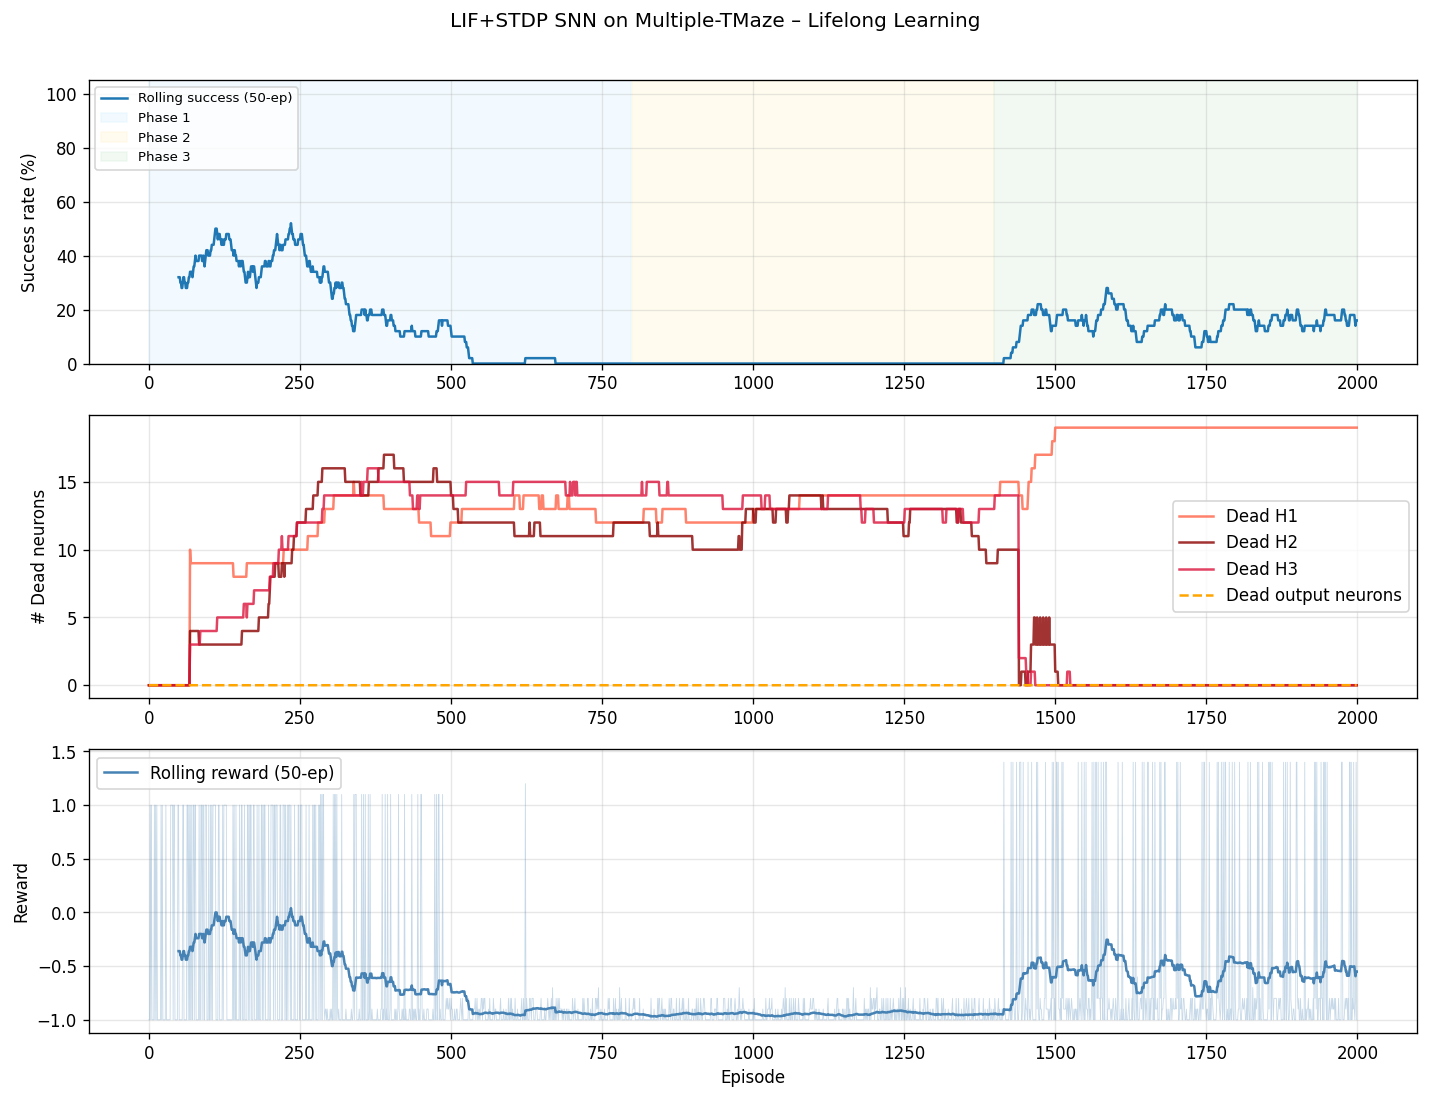
\includegraphics[width=0.8\linewidth]{fig5}
    \caption{隠れ層を三層に拡張した場合の正答率・Dead-Neuron数の推移} 
    \label{fig:fig5}
\end{figure}
結果としてデッドニューロン数は安定したものの、正答率は17\%〜20\%程で頭打ちとなった。
これは、ランダムに選ばれるゴールに対する偶然の正答確率（1/5 = 20\%）に等しく、入力からランダムなターゲットを予測することの根本的な限界を示している。
そこで次に、入力（ヒント）と報酬ゴール（ターゲット）の間に決定論的な法則性を持たせることにした。具体的には以下のルールを適用した：
\begin{equation}
\mathit{TargetGoal} = (\mathit{HintGoal} + 1) \pmod{5}
\end{equation}
この法則を適用してPhase1,2,3を再実行し、Wine-Towerの有無による比較を行った結果が図6である。
\begin{figure}[htbp]
    \centering
    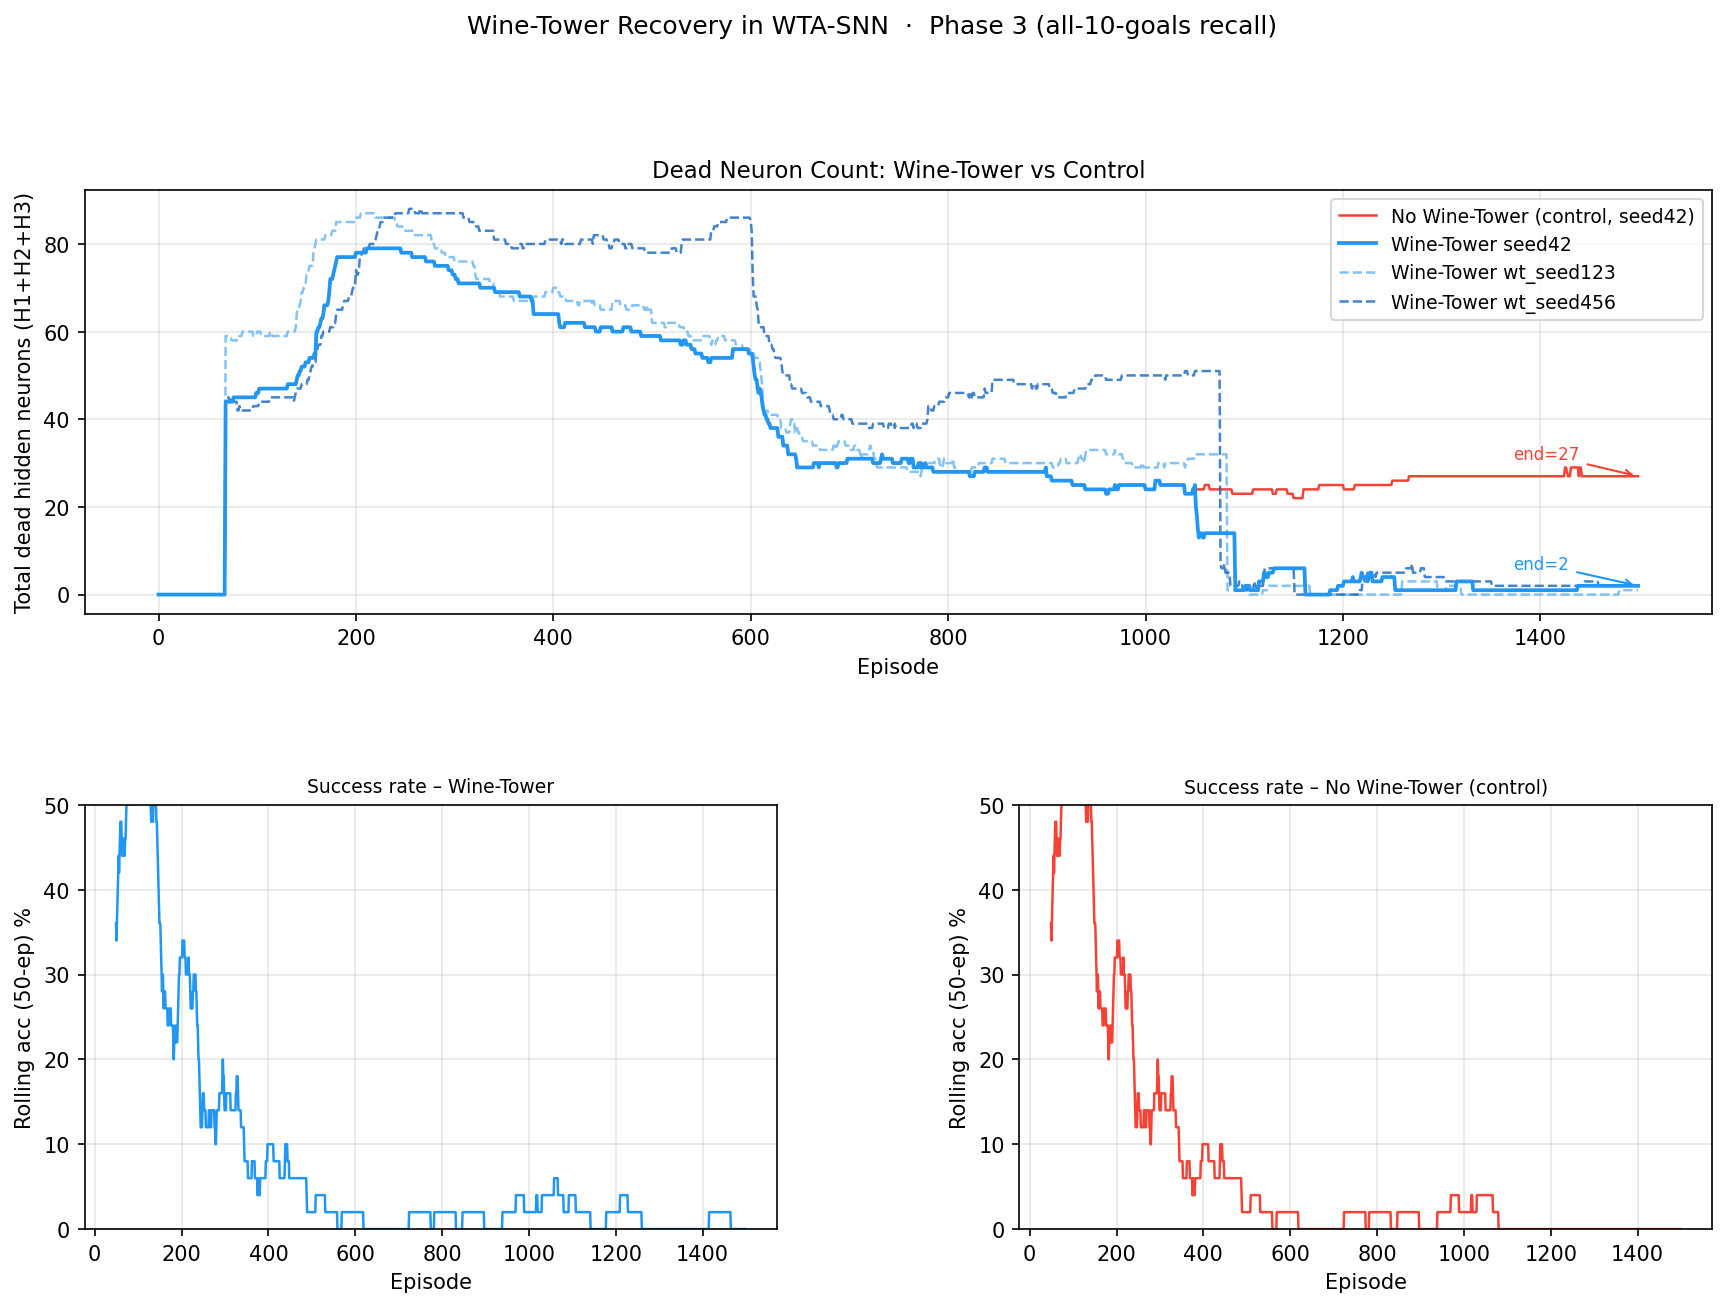
\includegraphics[width=0.8\linewidth]{fig6}
    \caption{決定論的ルール(Target=Hint+1)におけるWine-Towerとコントロールの比較} 
    \label{fig:fig6}
\end{figure}
グラフが示す通り、Wine-Towerを導入しないコントロール群（赤線）では、Phaseが進行するにつれてWTA競争に敗れたニューロンが永続的に死んだ状態となり、学習リソースが枯渇した。
一方、Wine-Towerを導入した群（青線）では、Phase 3において一度死んだニューロンがほぼ0個まで劇的に蘇生され、ネットワーク全体のリソースが新しい法則の学習に再動員されていることが確認できた。これにより、SNNの生涯学習における「Dead-Neuron問題」に対するWine-Towerモデルのリソース確保における有効性が強く示唆された。

しかし、機能的側面においては課題も残った。Wine-Towerによる強制的な蘇生とLTP強化は、休眠リソースの再利用には極めて優秀である反面、今回の実験では正答率を高い水準で維持し続けるには至らなかった。これは、蘇生されたニューロンが現在のタスクに対して急速に、かつ一斉に専門化する過程で、情報の均一化（Homogenization）を招き、ネットワーク全体の表現の多様性や既存の知識とのバランスが損なわれた可能性が考えられる。つまり、Wine-Towerはリソースの「量」を回復させる手段としては非常に強力であるが、それを機能的な「質」へと昇華させ、高いパフォーマンスを維持するためには、更なる重み制御の最適化が必要であることが明らかになった。

\bibliographystyle{plain}
\bibliography{references}
\end{document}
